% File name: datalogger/Reports/Interim_Report.tex
% Interim report for datalogger project
% Author: adh
% Date: Fri 17 May 2013 15:43

\documentclass[a4paper,11pt]{article}  % Standard document class
\usepackage[english]{babel}            % Set document language
\usepackage{fullpage}                  % Set up page for small margins etc

\usepackage{graphicx}                  % For including images in document
\usepackage{placeins}                  % Allows use of \FloatBarrier
% to avoid images or tables
% moving into next section
\usepackage{subfig}                    % For subfigures...

\usepackage{amsmath}                   % For improving maths/formula typesetting
\usepackage{tabularx}                  % Table changing package

\usepackage{algpseudocode}             % For producing algorithms/flowcharts
\usepackage{listings}                  % For including source code in document

\usepackage{url}

% Provide command for scientific notation
\providecommand{\e}[1]{\ensuremath{\times10^{#1}}}
\providecommand{\degrees}{\ensuremath{^{\circ}}}

% Define title here:
\title{Project SB3: Data Logger \\
       Interim Report \\
       Team 6}
\author{James Glanville\\
        jg597\\
        Emmanuel\\
        \and
        Andrew Holt\\
        ah635\\
        Emmanuel}
\date{20 May 2013}

\begin{document}

% generate title
\maketitle

\section{Introduction}

This project requires the development of a data logging embedded
system. It was decided to target parcel delivery as an application,
and to develop a system that could monitor the condition of a parcel
though transit. For this, it requires logging of temperature,
humidity, shock/impact and orientation. If time, we will also attempt
to monitor vibration. A prototype will be developed to show
functionality, but this system would need to be miniaturised for
real-world usage.

For the project, the circuit design was shared but overseen
primarily by James. Firmware is to be developed by James while Andrew
will develop the computer side software.

\section{Circuit Design}

\subsection{EEPROM and Accelerometer}

The EEPROM and the accelerometer will be connected to the I$^2$C bus
(I2C1) of the microcontroller. The resistor pullups are needed
because I$^2$C is open drain (Although the microcontroller does also have
optional internal pullups). The INT connector is used to signal to the
microcontroller that the accelerometer has registered an event. The
MM17660FC has a number of modes that can be configured to send an
interrupt when a sudden acceleration or change of orientation has
occurred. This will make the software more effective, as we will not
have to poll the accelerometer constantly. The circuit diagram is
shown in appendix \ref{sec:circuit-diagrams}, figure \ref{fig:i2cbus}.

\subsection{Humidity Sensor}

The humidity sensor responds to changes in humidity with a varying
capacitance. The principle of operation of the sensor circuit is as
follows: first, \texttt{CHARGE} is pulled low, to discharge the
capacitor. After a small delay it is pulled high, charging the
capacitor through the resistor. The microcontroller will poll the
\texttt{SENSE} pin, incrementing a counter, until \texttt{SENSE} reads
high. This counter value will be proportional to capacitance, and
hence humidity. To take repeated readings, the sensor is periodically
charged and discharged. This will not be quite as accurate as a
humidity sensor with digital or analogue output, but the low cost is
ideally suited to this project. The circuit diagram is shown in
appendix \ref{sec:circuit-diagrams}, figure \ref{fig:humcir}. The
design is based on one found online \cite{hum_sens}.

\subsection{Temperature Sensor}

The temperature is monitored using a thermistor. The conditioning
circuit is based on an example in \cite{HH}. The use of a series
10k$\Omega$ resistor gives very good linearity over a wide temperature
range, easily including that expected to be experienced by a parcel in
transit. The resistor values are chosen to give an op-amp output
voltage of $0\,\mathrm{V}$ at $-20\,\mathrm{\degrees C}$ and
$3.3\,\mathrm{V}$ at $50\,\mathrm{\degrees C}$. The op-amp used has
very good rail-rail operation, so may be run from a 3.3V with
negligible affect on performance (especially as extremes of temp are
unlikely to be experienced and at limits of reasonable linearity of
thermistor operation). The gain setting resistors may be knocked up a
decade if current draw from reference divider proves too high. The
circuit diagram is shown in appendix \ref{sec:circuit-diagrams},
figure \ref{fig:tempcond}.

\subsection{Voltage Regulator}

A $5\,\mathrm{V}$ regulator is being used to allow running from
batteries when in standalone mode. The circuit diagram is shown in
figure 

\section{Parts List}
\label{sec:parts-list}

The full parts list is shown in appendix
\ref{sec:full-parts-list}. The total cost is $\pounds 13.18$, but not
all of these will be used (bicolour LEDs came in pack of 5). Key
features are the accelerometer, EEPROM and LCD display.

\section{Communications}
\label{sec:communications}

2 way communication will be implemented between the computer and data
logging unit. The computer sends commands to the microcontroller and
the microcontroller sends data back to the computer.

\begin{figure}[!h]
  \begin{center}
    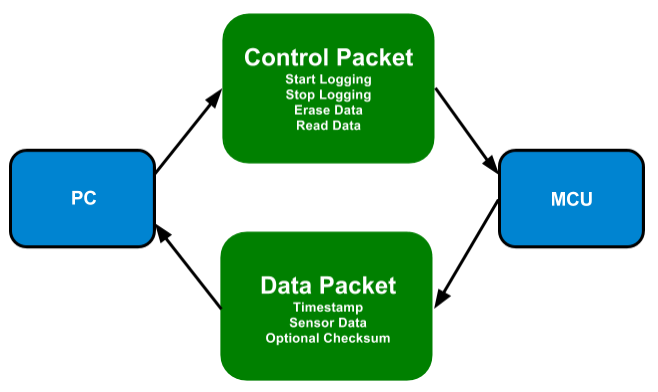
\includegraphics[width=0.8\textwidth]{comms_diagram.png}
  \end{center}
  \caption{Communications block diagram}
  \label{fig:commsdiag}
\end{figure}

\section{Firmware Design}
\label{sec:firmware-design}

At all times the microcontroller will be in one of the following
states:

\begin{itemize}
  \item Streaming to pc continuously.
  \item Standalone mode. Starts logging on button press.
  \item Transferring logged data to pc
  \item Command mode (Waiting for instruction such as EEPROM erase)
\end{itemize}

\section{Software Design}
\label{sec:software-design}

The software will require functions for communication with the
microcontroller and its own analysis and display routines. For
communication with the microcontroller, the following functions
will be required:
\begin{itemize}
  \item Start logging in linked mode.
  \item Stop logging in linked mode.
  \item Read data from standalone operation.
  \item Erase data.
\end{itemize}
The data related functions will be:
\begin{itemize}
  \item Ask for new data from MCU.
  \item Read in data when it arrives.
  \item Get all data from standalone operation.
  \item Add to data store (initially use an array/vector. If time
    allows, implement a database, allowing long term, high data storage).
  \item Find interest points (eg temp over/under given set level,
    shocks etc).
\end{itemize}
For display of data:
\begin{itemize}
  \item General GUI functions.
  \item Graph data (OpenGL?).
  \item Display interest points.
  \item Allow different views.
\end{itemize}

\newpage
\appendix

\section{Circuit Diagrams}
\label{sec:circuit-diagrams}

\begin{figure}[!h]
  \begin{center}
    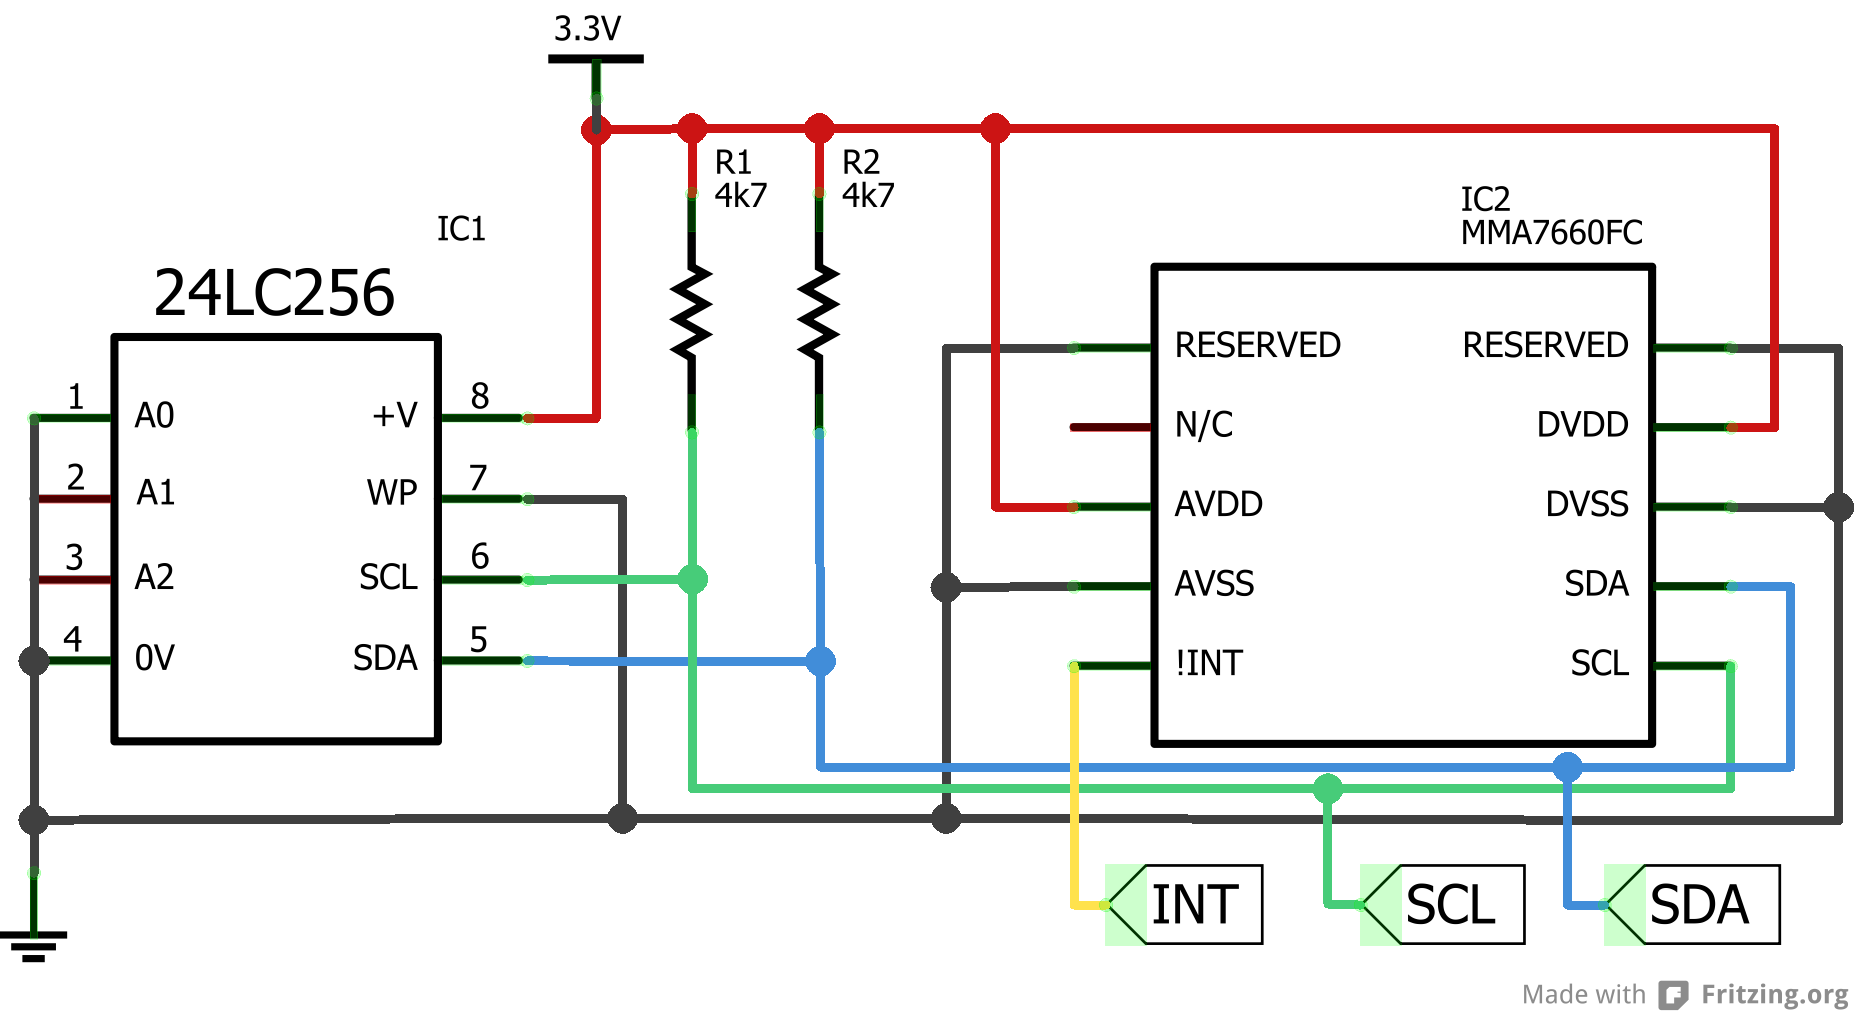
\includegraphics[width=0.8\textwidth]{i2c_schem.png}
  \end{center}
  \caption{EEPROM and accelerometer on I$^2$C Bus}
  \label{fig:i2cbus}
\end{figure}

\begin{figure}[!h]
  \begin{center}
    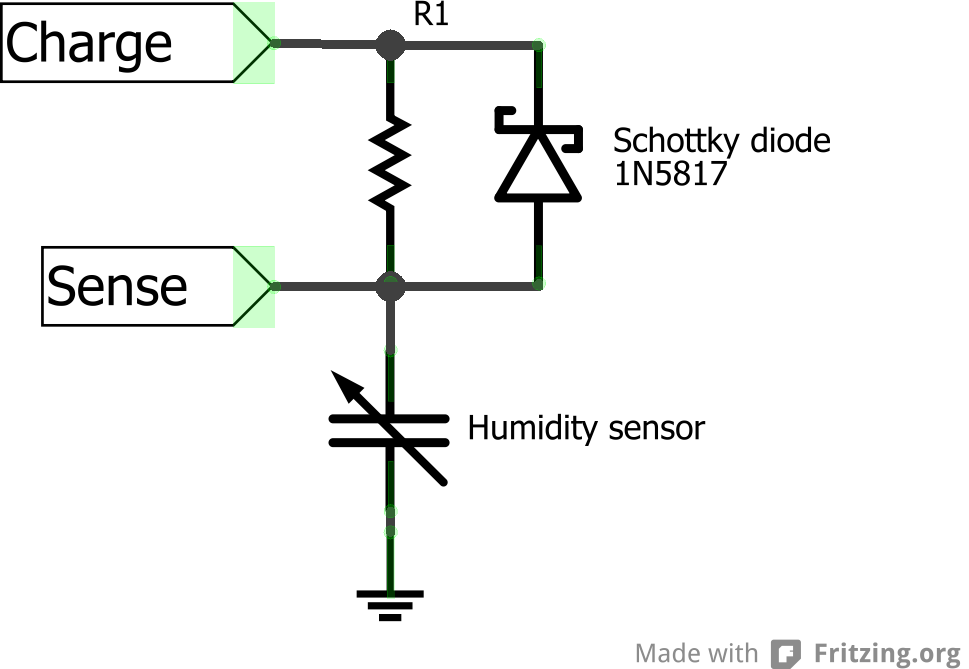
\includegraphics[width=0.5\textwidth]{humiditysensor_schem.png}
  \end{center}
  \caption{Measurement of humidity though varying capacitance}
  \label{fig:humcir}
\end{figure}

\begin{figure}[!h]
  \begin{center}
    \includegraphics[width=0.9\textwidth]{Thermistor_Conditioning_nonotes_schem.png}
  \end{center}
  \caption{Thermistor conditioning circuit}
  \label{fig:tempcond}
\end{figure}

\begin{figure}[!h]
  \begin{center}
    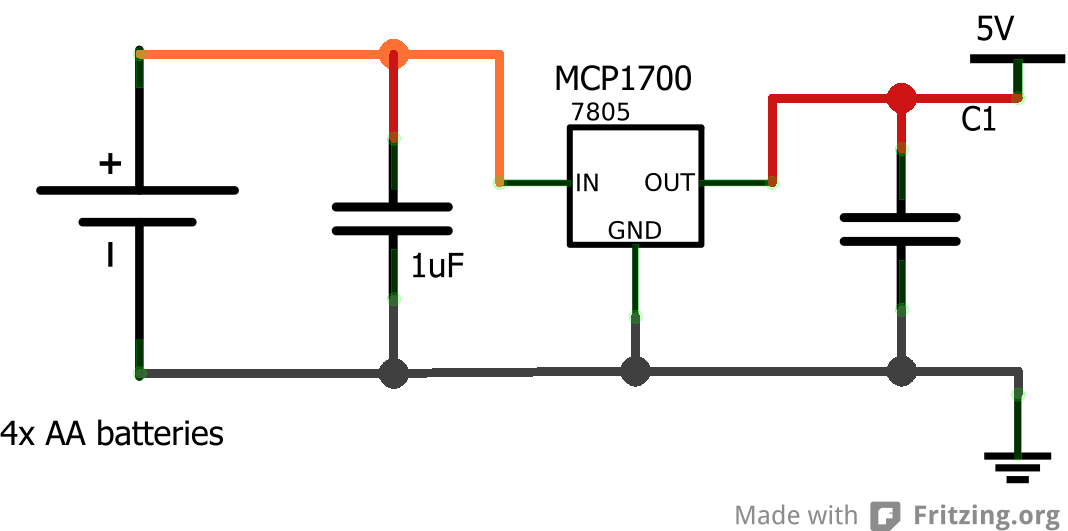
\includegraphics[width=0.6\textwidth]{power_schem.png}
  \end{center}
  \caption{Voltage Regulator}
  \label{fig:voltreg}
\end{figure}

\section{Full Parts List}
\label{sec:full-parts-list}

\begin{tabular}{llccc}
  Order Code & Description & Quantity & Unit price & Total Price \\
  \hline
  2238133 & Freescale 3-axis accelerometer & 2 & 0.97 & 1.94 \\
  1672384 & AUX NTC 10k thermistor & 1 & 0.20 & 0.20 \\
  1891432 & Multicomp humidity sensor & 1 & 2.08 & 2.08 \\
  2001770 & Kingbright bicolour LED & 5 & 0.159 & 0.80 \\
  1671493 & Powertip 8x2 lcd module & 1 & 3.40 & 3.40 \\
  9757970 & 256k eeprom & 1 & 0.80 & 0.80 \\
  1439438 & Microchip op-amp & 1 & 0.30 & 0.30 \\
  1650685 & Keystone 4xAA battery holder & 1 & 1.36 & 1.36 \\
  1712515 & Panasonic AA battery 4 pack & 1 & 1.94 & 1.94 \\
  1331481 & Microchip 5V regulator & 1 & 0.36 & 0.36 \\
  \hline
  &&& Total: & \pounds 13.18
\end{tabular}


\bibliographystyle{plain}
\bibliography{Interim_Report}

\end{document}